%%
%% Beginning of file 'sample61.tex'
%%
%% Modified 2016 September
%%
%% This is a sample manuscript marked up using the
%% AASTeX v6.1 LaTeX 2e macros.
%%
%% AASTeX is now based on Alexey Vikhlinin's emulateapj.cls 
%% (Copyright 2000-2015).  See the classfile for details.

%% AASTeX requires revtex4-1.cls (http://publish.aps.org/revtex4/) and
%% other external packages (latexsym, graphicx, amssymb, longtable, and epsf).
%% All of these external packages should already be present in the modern TeX 
%% distributions.  If not they can also be obtained at www.ctan.org.

%% The first piece of markup in an AASTeX v6.x document is the \documentclass
%% command. LaTeX will ignore any data that comes before this command. The 
%% documentclass can take an optional argument to modify the output style.
%% The command below calls the preprint style  which will produce a tightly 
%% typeset, one-column, single-spaced document.  It is the default and thus
%% does not need to be explicitly stated.
%%
%%
%% using aastex version 6.1
\documentclass[twocolumn]{aastex62}

%% The default is a single spaced, 10 point font, single spaced article.
%% There are 5 other style options available via an optional argument. They
%% can be envoked like this:
%%
%% \documentclass[argument]{aastex61}
%% 
%% where the arguement options are:
%%
%%  twocolumn   : two text columns, 10 point font, single spaced article.
%%                This is the most compact and represent the final published
%%                derived PDF copy of the accepted manuscript from the publisher
%%  manuscript  : one text column, 12 point font, double spaced article.
%%  preprint    : one text column, 12 point font, single spaced article.  
%%  preprint2   : two text columns, 12 point font, single spaced article.
%%  modern      : a stylish, single text column, 12 point font, article with
%% 		  wider left and right margins. This uses the Daniel
%% 		  Foreman-Mackey and David Hogg design.
%%
%% Note that you can submit to the AAS Journals in any of these 6 styles.
%%
%% There are other optional arguments one can envoke to allow other stylistic
%% actions. The available options are:
%%
%%  astrosymb    : Loads Astrosymb font and define \astrocommands. 
%%  tighten      : Makes baselineskip slightly smaller, only works with 
%%                 the twocolumn substyle.
%%  times        : uses times font instead of the default
%%  linenumbers  : turn on lineno package.
%%  trackchanges : required to see the revision mark up and print its output
%%  longauthor   : Do not use the more compressed footnote style (default) for 
%%                 the author/collaboration/affiliations. Instead print all
%%                 affiliation information after each name. Creates a much
%%                 long author list but may be desirable for short author papers
%%
%% these can be used in any combination, e.g.
%%
%% \documentclass[twocolumn,linenumbers,trackchanges]{aastex61}

%% AASTeX v6.* now includes \hyperref support. While we have built in specific
%% defaults into the classfile you can manually override them with the
%% \hypersetup command. For example,
%%
%%\hypersetup{linkcolor=red,citecolor=green,filecolor=cyan,urlcolor=magenta}
%%
%% will change the color of the internal links to red, the links to the
%% bibliography to green, the file links to cyan, and the external links to
%% magenta. Additional information on \hyperref options can be found here:
%% https://www.tug.org/applications/hyperref/manual.html#x1-40003

%% If you want to create your own macros, you can do so
%% using \newcommand. Your macros should appear before
%% the \begin{document} command.
%%
\usepackage{multirow, amsmath}
\newcommand{\vdag}{(v)^\dagger}
\newcommand\aastex{AAS\TeX}
\newcommand\latex{La\TeX}
\newcommand{\sm}{M_\odot}
\newcommand{\sr}{R_\odot}

%% Reintroduced the \received and \accepted commands from AASTeX v5.2
\received{\today}
\revised{}
\accepted{}
%% Command to document which AAS Journal the manuscript was submitted to.
%% Adds "Submitted to " the arguement.
\submitjournal{PASP}

%% Mark up commands to limit the number of authors on the front page.
%% Note that in AASTeX v6.1 a \collaboration call (see below) counts as
%% an author in this case.
%
%\AuthorCollaborationLimit=3
%
%% Will only show Schwarz, Muench and "the AAS Journals Data Scientist 
%% collaboration" on the front page of this example manuscript.
%%
%% Note that all of the author will be shown in the published article.
%% This feature is meant to be used prior to acceptance to make the
%% front end of a long author article more manageable. Please do not use
%% this functionality for manuscripts with less than 20 authors. Conversely,
%% please do use this when the number of authors exceeds 40.
%%
%% Use \allauthors at the manuscript end to show the full author list.
%% This command should only be used with \AuthorCollaborationLimit is used.

%% The following command can be used to set the latex table counters.  It
%% is needed in this document because it uses a mix of latex tabular and
%% AASTeX deluxetables.  In general it should not be needed.
%\setcounter{table}{1}

%%%%%%%%%%%%%%%%%%%%%%%%%%%%%%%%%%%%%%%%%%%%%%%%%%%%%%%%%%%%%%%%%%%%%%%%%%%%%%%%
%%
%% The following section outlines numerous optional output that
%% can be displayed in the front matter or as running meta-data.
%%
%% If you wish, you may supply running head information, although
%% this information may be modified by the editorial offices.
\shorttitle{PS1 Star-galaxy Catalog}
\shortauthors{One then the other}
%%
%% You can add a light gray and diagonal water-mark to the first page 
%% with this command:
\watermark{DRAFT}
%% where "text", e.g. DRAFT, is the text to appear.  If the text is 
%% long you can control the water-mark size with:
%  \setwatermarkfontsize{dimension}
%% where dimension is any recognized LaTeX dimension, e.g. pt, in, etc.
%%
%%%%%%%%%%%%%%%%%%%%%%%%%%%%%%%%%%%%%%%%%%%%%%%%%%%%%%%%%%%%%%%%%%%%%%%%%%%%%%%%

%%%%%%%%%%%%%%%%%%%%%%%%%%%%%%%%%%%%%%%%%%%%%%%%%%%%%%%%%%%%%%%%%%%%%%%%%%%%%%%%
%%
%% The following section defines new commands for comments from co-authors
%%
\newcommand{\yutaro}[1]{{\color{red} yt: {#1}}}
\newcommand{\NC}[1]{{\color{brown} NC: {#1}}}
\newcommand{\aam}[1]{{\color{blue} aam: {#1}}}
\newcommand{\todo}[1]{{\color{magenta} to-do: {#1}}}
%%
%%%%%%%%%%%%%%%%%%%%%%%%%%%%%%%%%%%%%%%%%%%%%%%%%%%%%%%%%%%%%%%%%%%%%%%%%%%%%%%%

%% This is the end of the preamble.  Indicate the beginning of the
%% manuscript itself with \begin{document}.

\begin{document}

\title{\textbf{something better needed} A PanSTARRS1 Star--Galaxy Model: Application in the ZTF Real-Time Pipeline}

%% LaTeX will automatically break titles if they run longer than
%% one line. However, you may use \\ to force a line break if
%% you desire. In v6.1 you can include a footnote in the title.

%% A significant change from earlier AASTEX versions is in the structure for 
%% calling author and affilations. The change was necessary to implement 
%% autoindexing of affilations which prior was a manual process that could 
%% easily be tedious in large author manuscripts.
%%
%% The \author command is the same as before except it now takes an optional
%% arguement which is the 16 digit ORCID. The syntax is:
%% \author[xxxx-xxxx-xxxx-xxxx]{Author Name}
%%
%% This will hyperlink the author name to the author's ORCID page. Note that
%% during compilation, LaTeX will do some limited checking of the format of
%% the ID to make sure it is valid.
%%
%% Use \affiliation for affiliation information. The old \affil is now aliased
%% to \affiliation. AASTeX v6.1 will automatically index these in the header.
%% When a duplicate is found its index will be the same as its previous entry.
%%
%% Note that \altaffilmark and \altaffiltext have been removed and thus 
%% can not be used to document secondary affiliations. If they are used latex
%% will issue a specific error message and quit. Please use multiple 
%% \affiliation calls for to document more than one affiliation.
%%
%% The new \altaffiliation can be used to indicate some secondary information
%% such as fellowships. This command produces a non-numeric footnote that is
%% set away from the numeric \affiliation footnotes.  NOTE that if an
%% \altaffiliation command is used it must come BEFORE the \affiliation call,
%% right after the \author command, in order to place the footnotes in
%% the proper location.
%%
%% Use \email to set provide email addresses. Each \email will appear on its
%% own line so you can put multiple email address in one \email call. A new
%% \correspondingauthor command is available in V6.1 to identify the
%% corresponding author of the manuscript. It is the author's responsibility
%% to make sure this name is also in the author list.
%%
%% While authors can be grouped inside the same \author and \affiliation
%% commands it is better to have a single author for each. This allows for
%% one to exploit all the new benefits and should make book-keeping easier.
%%
%% If done correctly the peer review system will be able to
%% automatically put the author and affiliation information from the manuscript
%% and save the corresponding author the trouble of entering it by hand.

\correspondingauthor{A.~A.~Miller}
\email{amiller@northestern.edu}

% \author[0000-0001-9515-478X]{A.~A.~Miller}
% \affil{Center for Interdisciplinary Exploration and Research in Astrophysics (CIERA) and Department of Physics and Astronomy, Northwestern University, 2145 Sheridan Road, Evanston, IL 60208, USA}
% \affil{The Adler Planetarium, Chicago, IL 60605, USA}

\author{Concerned ZTF Scientists}
\affil{Zwicky Transient Facility}

%% Note that the \and command from previous versions of AASTeX is now
%% depreciated in this version as it is no longer necessary. AASTeX 
%% automatically takes care of all commas and "and"s between authors names.

%% AASTeX 6.1 has the new \collaboration and \nocollaboration commands to
%% provide the collaboration status of a group of authors. These commands 
%% can be used either before or after the list of corresponding authors. The
%% argument for \collaboration is the collaboration identifier. Authors are
%% encouraged to surround collaboration identifiers with ()s. The 
%% \nocollaboration command takes no argument and exists to indicate that
%% the nearby authors are not part of surrounding collaborations.

%% Mark off the abstract in the ``abstract'' environment. 
\begin{abstract}

We did a decent job of separating stars and galaxies.

\end{abstract}

%% Keywords should appear after the \end{abstract} command. 
%% See the online documentation for the full list of available subject
%% keywords and the rules for their use.
\keywords{catalogs --- galaxies: statistics --- methods: data analysis --- methods: statistical --- stars: statistics --- surveys}

%% From the front matter, we move on to the body of the paper.
%% Sections are demarcated by \section and \subsection, respectively.
%% Observe the use of the LaTeX \label
%% command after the \subsection to give a symbolic KEY to the
%% subsection for cross-referencing in a \ref command.
%% You can use LaTeX's \ref and \label commands to keep track of
%% cross-references to sections, equations, tables, and figures.
%% That way, if you change the order of any elements, LaTeX will
%% automatically renumber them.

%% We recommend that authors also use the natbib \citep
%% and \citet commands to identify citations.  The citations are
%% tied to the reference list via symbolic KEYs. The KEY corresponds
%% to the KEY in the \bibitem in the reference list below. 

\section{Introduction}\label{sec:intro}

\yutaro{I've restructured the intro, I think we should pitch the paper as PS1
catalog used by ZTF, rather than ZTF project. That way other people will
hopefully use the catalog even if they do not use ZTF.}

The proliferation of wide-field optical detectors has led to a plethora of
imaging catalogs in the past two decades. \yutaro{I think we should add some
general text here about the importance of separating stars and galaxies here
- do you want to take the first effort for that?}
\NC{
Separating point sources (mostly stars) from extended sources (galaxies), 
especially in faint samples, 
is one of the most challenging and important steps in the 
extraction of sensitive astronomical information 
from such imaging catalogs, 
and boosts the progress in our understanding for the universe. 
The characteristic of dark matter can be investigated 
by tracing the structure in the Milky Way halo ({\it e.g.}, \citealt{Belokurov06}), 
measuring galaxy-galaxy correlation functions ({\it e.g.}, \citealt{Ross11, Ho15})
including dwarf galaxies that can be searched by stellar overdensities \citep{Belokurov07}, 
and detecting the weak lensing signal from cosmic shear \citep{Soumagnac15}. 
The number count density of galaxies as a function of luminosity (luminosity function) 
can be used for the assessment of the geometry of the universe \citep{Yasuda01} 
and the theory of galaxy formation ({\it e.g.}, \citealt{Loveday12, Moorman15}). 
}

Given the many applications for a catalog that separates point sources from
galaxies, we turn our attention to the wide-field Pan-STARRS1 (PS1) survey
\citep{Chambers16}, whose 3$\pi$ survey provides a felicitous data set.

The 1.8\,m PS1 telescope is equipped with a wide-field ($\sim$7\,deg$^2$) 1.4
gigapixel camera and is located at Haleakala Observatory in Hawaii
\citep{Hodapp04}. PS1 primarily uses five broadband filters,
$g_{\mathrm{P1}}$, $r_{\mathrm{P1}}$, $i_{\mathrm{P1}}$, $z_{\mathrm{P1}}$,
and $y_{\mathrm{P1}}$ (hereafter $grizy_{\mathrm{P1}}$). The PS1 3$\pi$
survey scanned the entire visible sky ($\mathrm{Dec.}>-30^\circ$) 60 times in
the five filters over a four-year time span \citep{Chambers16}. This repeated
imaging was used to create deep stacks \citep{Magnier16b}, with a typical
5$\sigma$ depth of $\sim$23.2\,mag with a median seeing of $1.19\arcsec$ in
the $r$-band \citep{Tonry12, Schlafly12, Chambers16}. The first PS1 data
release (DR1) provides flux and pixel-based shape measurements for $>$3
billion sources \citep{Flewelling16}.

Our aim is to develop a large, deep catalog of stars (point sources) and
galaxies using PS1 data. The catalog is to be general purpose, however, our
immediate goal is to support the real-time search for transients in the
Zwicky Transient Facility (ZTF; \citealt{Bellm18}). Previously, a similar
catalog was developed using Palomar Transient Factory (PTF) data
\citep{Miller17}. 

The PTF star--galaxy catalog was developed using \texttt{SExtractor}
\citep{bertin96} flux and shape measurements made on deep stacks of PTF
imaging. Stars and galaxies were separated using a machine learning
methodology utilizing the random forest (RF) algorithm \citep{Breiman01}.
Briefly, supervised machine learning methods build a non-parametric mapping
between \textit{features}, measured properties, and \textit{labels}, the
target classification, via a training set. The training set contains sources
for which the labels are already known, facilitating the construction of a
features to labels mapping. Following this training, the machine learning
model can produce predictions on new observations where the labels are
unknown.

The PTF point-source catalog was constructed to support the real-time search
for electromagetic counterparts to gravitational wave events. Given that
these events are expected to be very rare (\todo{citation}), the figure of
merit (FoM) for the PTF model was defined as the true positive rate
(corresponding to the fraction of stars that are correctly classified) at a
fixed false positive rate (fraction of galaxies that are misclassified) equal
to 0.005 \citep{Miller17}. While the PTF point-source catalog includes
$\sim$1.7$\times 10^8$ objects, it is expected that a full
$\sim$8$\times10^7$ point sources are excluded as false negatives
\citep{Miller17}.

A star--galaxy separation model built on PS1 data will produce dramatic
improvements over the PTF catalog. PS1 observations are deeper, feature
better seeing, and include 5 filters (the PTF catalog was built with
observations in a single filter, $R_\mathrm{PTF}$). Additionally, one of the
12 CCDs in the PTF camera did not work \citep{Law09}, meaning $\sim$8\% of
the sky above $\mathrm{Dec.} = 30^\circ$ has no classifications in the PTF
catalog.

Here, we construct a new star--galaxy separation model using PS1 DR1 data in
conjunction with a new machine learning methodology. The model is trained
using \textit{Hubble Space Telescope} observations, which should provide an
improvement over the Sloan Digital Sky Survey (SDSS; \citealt{York00})
spectroscopic training set used in \citet{Miller17}. As in \citet{Miller17},
we use the RF algorithm to separate point sources and extended sources. Our
new PS1 model outperforms alternatives and has already been incorporated into
the ZTF real-time pipeline.

\todo{Need to add something about optimizing the same FoM as the first Miller paper}

%%%
\if0
The system comprises a 1.8 m primary and 0.9 m secondary mirrors \citep{Hodapp04}, 
produces a field of view of 3.3 deg$^2$ with 60 CCD chips each of 4800$\times$4800 pixels, 
and the pixel resolution is 0.258 arcsec pixel$^{-1}$ at the focal plane. 
The filter system consists of five main broadband filters, 
$g_{\mathrm{P1}}$, $r_{\mathrm{P1}}$, $i_{\mathrm{P1}}$, $z_{\mathrm{P1}}$, and $y_{\mathrm{P1}}$, 
and that effective wavelength is 481 nm, 617 nm, 752 nm, 866 nm, and 962 nm, 
respectively \citep{Tonry12, Schlafly12}. 
The typical 5$\sigma$ depth of stack image is 23.3, 23.2, 23.1, 22.3, and 21.3 mag 
white that of a single epoch is 22.0, 21.8, 21.5, 20.9, and 19.7 mag in the AB system, 
with a median seeing of 1.31, 1.19, 1.11, 1.07, and 1.02 arcsec, respectively \citep{Chambers16}. 
\fi
%%%


\section{Model Data}\label{sec:model_data}

Data for the star-galaxy model were obtained from the PS1 casjobs
server.\footnote{\url{http://mastweb.stsci.edu/ps1casjobs/home.aspx}} The PS1
database provides flux measurements via aperture photometry,
point-spread-function (PSF) photometry, and \citet{Kron80}
photometry.\footnote{A subset of bright sources ($i < 21\,\mathrm{mag}$)
outside the Galactic plane have additional photometric measurements, e.g.,
exponential or \citet{Sersic63} profiles, in the \textit{StackModelFitExp} and
\textit{StackModelFitSer} tables, respectively. We ignore these measurements
for this study as they are not available for all sources.} These flux
measurements are produced by PS1 in 3 different ways. The mean brightness
measured on the individual PS1 frames is reported in the \textit{MeanObject}
table, the mean brightness measured via forced-PSF/aperture photometry on the
individual PS1 frames is reported in the \textit{ForcedMeanObject} table, and
finally, the brightness measured on the full-depth stacked PS1 images is
reported in the \textit{StackObjectThin} table. The
\textit{StackObjectAttributes} table further supplements these tables with
point-source object shape measurements, which prove useful to discriminate
stars and galaxies. Ultimately, see \S\ref{sec:simple_model}, we use flux
measurements from the \textit{StackObjectThin} table and shape measurements
from the \textit{StackObjectAttributes} to build our models.

\subsection{The \textit{HST} Training Set} \label{sec:hst_train}

A fundamental challenge in the construction of any supervised machine learning
model is the curation of a high-fidelity training set. A subset of the data
that requires classification must have known labels so the machine can learn
the proper mapping between features and labels. The superior image quality of
the \textit{Hubble Space Telescope} (\textit{HST}) provides exceptionally
accurate morphological classifications, making it an ideal source of a training
set for lower quality ground-based imaging (e.g., \citealt{Lupton01}). The
downside of \textit{HST} is that the field of view is relatively small, so it
is difficult to construct a large and diverse training set suitable for
predictions over the entire sky.

We use the largest contiguous area imaged by \textit{HST}, the 1.64\,deg$^2$
COSMOS field, to construct a training set for our models. Morphological
classifications of \textit{HST} COSMOS sources are provided in
\citet{Leauthaud07}. \citeauthor{Leauthaud07} demonstrate reliable
classifications to $\sim$25\,mag, which is significantly deeper than the
faintest sources detected by PS1. We identify counterparts in the PS1 and
\textit{HST} data by performing a spatial crossmatch between the two catalogs
using a 1\arcsec radius.\footnote{This matching radius is the same employed
by PS1 to associate individual detections in the \textit{MeanObject} table
with detections in the \textit{StackObjectAttributes} table.} We further
excluded sources from the \citet{Leauthaud07} catalog with
$\texttt{MAG\_AUTO} > 25$\,mag, as these sources are too faint to be detected
by PS1 meaning their crossmatch counterparts are likely spurious. Following
this procedure, we find that there are 87,431 sources in the
\citet{Leauthaud07} catalog with PS1 counterparts. Of these, 80,974 are
unique in that there is a one-to-one correspondence between \textit{HST}
source and a single PS1 \textit{ObjID}. The training set is further reduced
to 75,927 once our detection criteria are applied (see
\S\ref{sec:simple_model}), and, of those, only 47,093 have
$\texttt{nDetections} \ge 1$ in the PS1 database (hereafter, the \textit{HST}
training set).\footnote{$\texttt{nDetections}$ refers to the number of
detections in individual PS1 exposures. Thus, \textit{StackObjectThin} souces
can have $\texttt{nDetections}$ = 0 if they are only detected in the PS1
stack images.}

\subsection{The SDSS Training Set}\label{sec:sdss}

\begin{figure*}[htb]
 \centering
  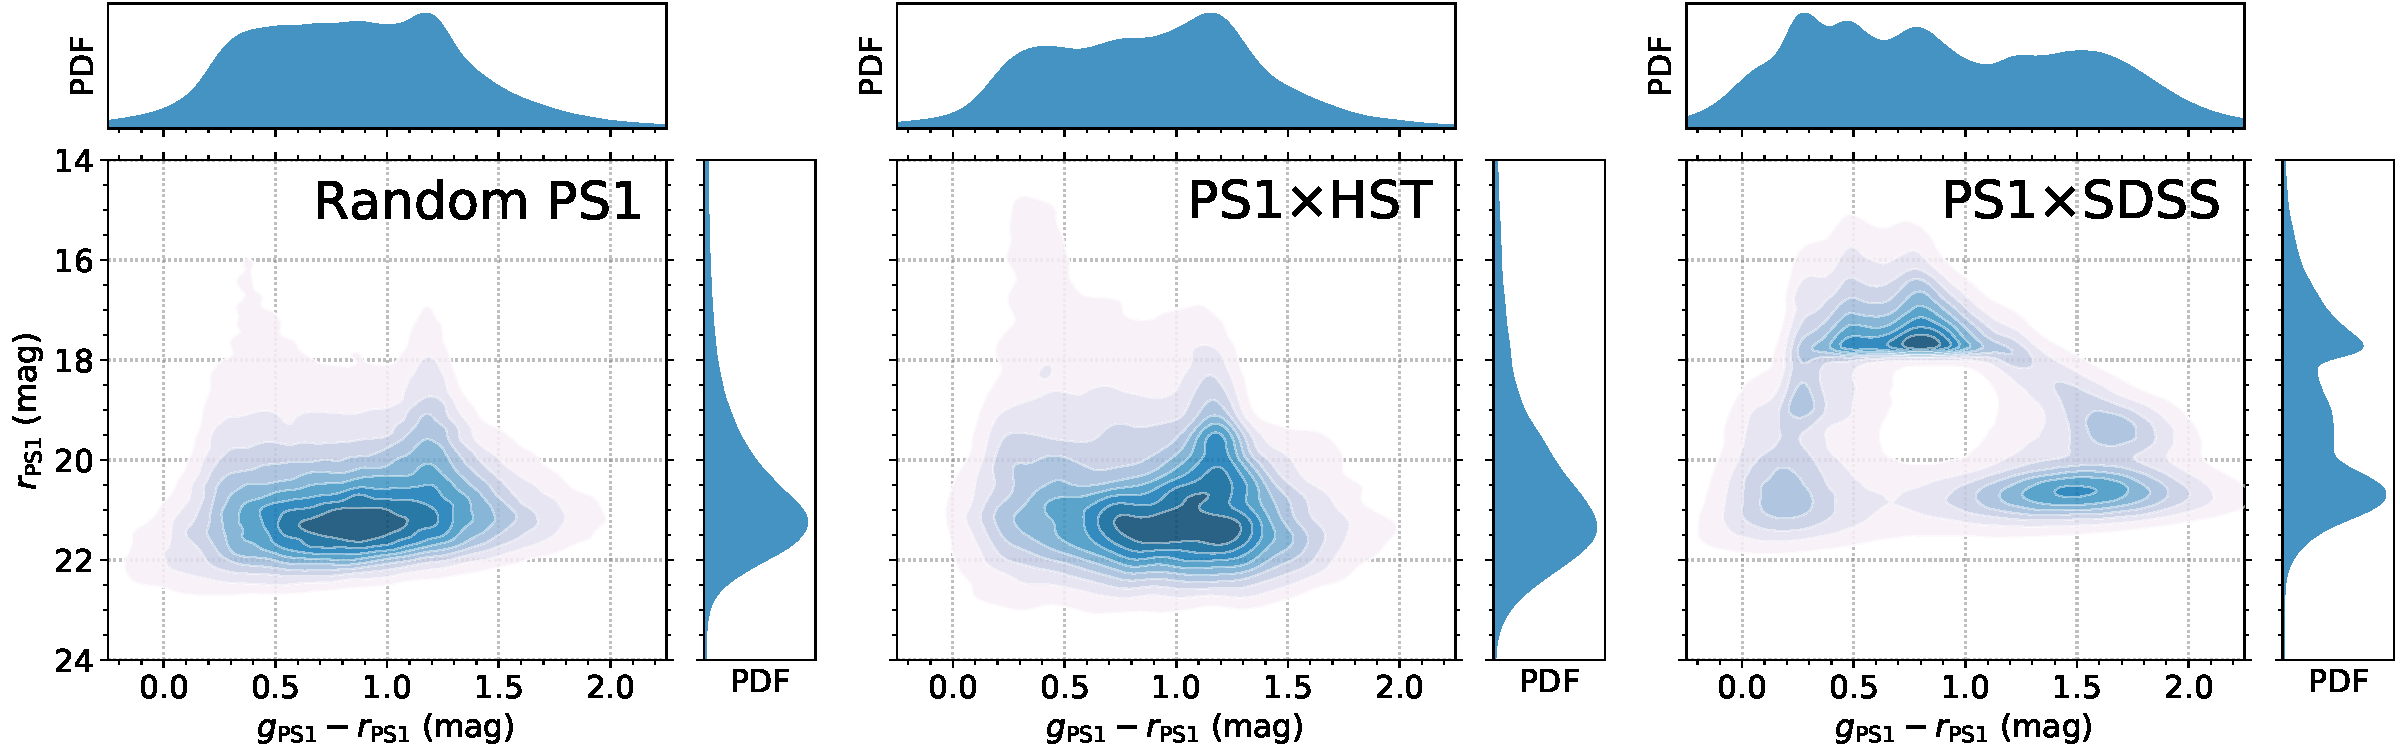
\includegraphics[width=7.2in
  %,bb = 0 0 1152 360
  ]{./Figures/ColorMagDiagram.pdf}
  \caption{
  PS1 color-magnitude diagrams for \textit{left}: $10^6$ randomly selected sources, \textit{center}: the \textit{HST} training set, and \textit{right}: the SDSS training set. The primary panels show a two-dimensional (2D) Gaussian kernel density estimate (KDE) of the probability density function (PDF) of each subset of sources in the $r_\mathrm{PS1}$--$g_\mathrm{PS1} - r_\mathrm{PS1}$ plane. The shown contour levels extend from 0.9 to 0.1 in 0.1 intervals. To the top and right of the primary panels are marginalized 1D KDEs of the PDF for the $g_\mathrm{PS1} - r_\mathrm{PS1}$ color and $r_\mathrm{PS1}$ brightness, respectively. Kron aperture measurements from the \textit{StackObjectThin} table are used to estimate each of the PDFs. \yutaro{Is this last sentence correct?: Yes. }
  }
  %
  \label{fig:cmd}
\end{figure*}

The SDSS spectroscopic catalog classifies everything it observes as either a
star, galaxy, or quasi-stellar object (QSO). Using a $1\arcsec$ cross-match
radius, we find 3,822,297 sources with SDSS optical spectra have PS1
counterparts (hereafter, the SDSS training set). Thus, with an orders of
magnitude larger training set, and spectroscopic classifications that should
be pristine and superior to mophological clsasifications, one might expect
the SDSS training set to be optimal for training the machine learning model.
However, as noted in \citep{Miller17}, the SDSS spectroscopic targeting
algorithms were highly biased, and as a result prove challenging as a
training set.

Color-magnitude diagrams (CMDs) of the \textit{HST} and SDSS training sets
are compared to a random selection of $10^6$ sources from the PS1 database in
Figure~\ref{fig:cmd}. It is clear from Figure~\ref{fig:cmd} that the SDSS
training set is completely different from typical sources in PS1 and that
there are few SDSS sources in the highest density regions of the PS1 CMD.
Given the stark mismatch between typical PS1 sources and the SDSS training
set, we adopt the \textit{HST} training set for the development of our model.
We retain the SDSS training set as an independent test set to assess the
accuracy of the model following construction.

\section{Model Features}\label{sec:model_features}

In addition to developing a training set, we must select features to use as an input for the model. As noted in \S\ref{sec:model_data}, the PS1 database provides flux and shape measurements in each of the $grizy_\mathrm{PS1}$ filters. Adopting each of these measurements as features for the model presents a significant problem: missing data. There are relatively few sources in the PS1 database that are detected in all 5 filters. Typically, to cope with missing data one can either (i) remove sources detected in fewer than 5 filters, or (ii) assign some value, via either imputation (e.g., \citealt{Miller17}) or the use of a dummy variable, to the missing data. Given that the vast majority of PS1 sources are faint and are not detected in all 5 filters, neither of these possiblities is attractive for our present purposes.

Rather than use the raw features from the database, we engineer a series of ``white flux'' features that combine the relevant measurements across all filters in which a source is detected. In a given filter, a source is detected if the $\mathtt{PSFFlux}_f$, $\mathtt{KronFlux}_f$, and $\mathtt{ApFlux}_f$ are \textit{all $> 0$}, where the $f$ subscript refers to a specific filter. The ``white flux'' feature is then created as:
%
\begin{equation}
    \mathtt{white[Feat]} =  \frac{\sum_f^{f = grizy_\mathrm{PS1}} w_f  \, \mathtt{Feat}_f \, \mathrm{det}_f}{\sum_f^{f = grizy_\mathrm{PS1}} w_f}, 
\end{equation}
%
where the sum is over the 5 PS1 filters, \texttt{Feat} is the feature from the \textit{StackObjectAttributes} table, $\mathrm{det}_f = 1$ if the source is detected in the $f$ filter, as defined above, or $\mathrm{det}_f = 0$ if not detected, and $w_f$ is the weight assigned to each filter:
%
\begin{equation}
    w_f = \left(\frac{\mathtt{KronFlux}_f}{\mathtt{KronFluxErr}_f}\right)^2,
\end{equation}
%
equivalent to signal-to-noise ratio (SNR) squared in the given filter. Ultimately, the ``white flux'' features correspond to a weighted mean, with weights equal to the square of the SNR. 

Our final model includes 11 ``white flux'' features to separate stars and
galaxies. The database features include: \texttt{PSFFlux},\footnote{For the
\texttt{PSFFlux} feature $w_f =
(\mathtt{PSFFlux}_f/\mathtt{PSFFluxErr}_f)^2$.} \texttt{KronFlux},
\texttt{ApFlux},\footnote{For the \texttt{ApFlux} feature $w_f =
(\mathtt{ApFlux}_f/\mathtt{ApFluxErr}_f)^2$ 
\NC{I think we used $w_f =
(\mathtt{PSFFlux}_f/\mathtt{PSFFluxErr}_f)^2$ for \texttt{ApFlux} 
because of the superior performance of \texttt{whitePSFApRatio}}. 
} \texttt{ExtNSigma},
\texttt{KronRad}, \texttt{psfChiSq}, \texttt{psfLikelihood},
\texttt{momentYY}, \texttt{momentXY}, \texttt{momentXX}, and
\texttt{momentRH}.\footnote{Prior to their ``white flux'' calculation the
shape features (\texttt{KronRad}, \texttt{momentYY}, \texttt{momentXY},
\texttt{momentXX}, and \texttt{momentRH}) are normalized by the seeing in the
respective bandpass, which we define as the \texttt{psfMajorFWHM} and
\texttt{psfMinorFWHM} added in quadrature. \texttt{KronRad} has units of
arcsec, \texttt{momentRH} has units of arcsec$^{0.5}$, and the remaining
shape features have units of arcsec$^{2}$. They are each normalized by
dividing by the seeing raised to the appropriate power. } The remaining
features in the database were either uninformative or would bias the model,
such as R.A.\ and Dec.\ (see e.g., \citealt{Richards12a}). We do not directly
include \texttt{whitePSFFlux}, \texttt{whiteKronFlux}, and
\texttt{whiteApFlux} in the model. We found that the inclusion of these
features resulted in a bias whereby all sources brighter than $\sim$16\,mag
were automatically classified as stars. Instead, we include the ratio of the
different flux measures: \texttt{whitePSFKronRatio} =
\texttt{whitePSFFlux}/\texttt{whiteKronFlux}, \texttt{whitePSFApRatio} =
\texttt{whitePSFFlux}/\texttt{whiteApFlux}, as well as a third feature
\texttt{whitePSFKronDist} (see \S\ref{sec:simple_model}).

As we previously alluded to, the primary benefit of the ``white flux''
features is that they can be calculated for every source in PS1 thus allowing
each to be compared on common ground. Furthermore, the SNR for the ``white
flux'' features is greater than the SNR for the equivalent feature in a
single filter. The downside of these features is that for some sources,
especially at the bright end, color information is lost. While a blue source
and red source with identical \texttt{whitePSFFlux} values are intrinsically
very different, the ``white flux'' features obscure that information for the
classifier. Ultimately, we tested models with and without the ``white flux''
features and found that they are statistically equivalent when tested with
the \textit{HST} training set.

The direct use of color information as model features would require reddening
corrections for all PS1 sources. Not only is this a daunting task, but
accurate corrections would require a priori knowledge as to which sources are
Galactic and which are extragalactic (e.g., \citealt{Green15}). The PS1
catalog is being developed precisely to answer this question. Furthermore,
the pencil beam sample from the \textit{HST} training set traces a narrow
range of dust columns, so the application of a model including color
information without reddening corrections would lead to biased
classifications, particularly in regions of high reddening (e.g., the
Galactic plane). We conclude that the benefits of the ``white flux''
features, which eliminate the need for reddening corrections, outweigh any
losses from the exclusion of color information.

\begin{figure*}[htb]
 \centering
  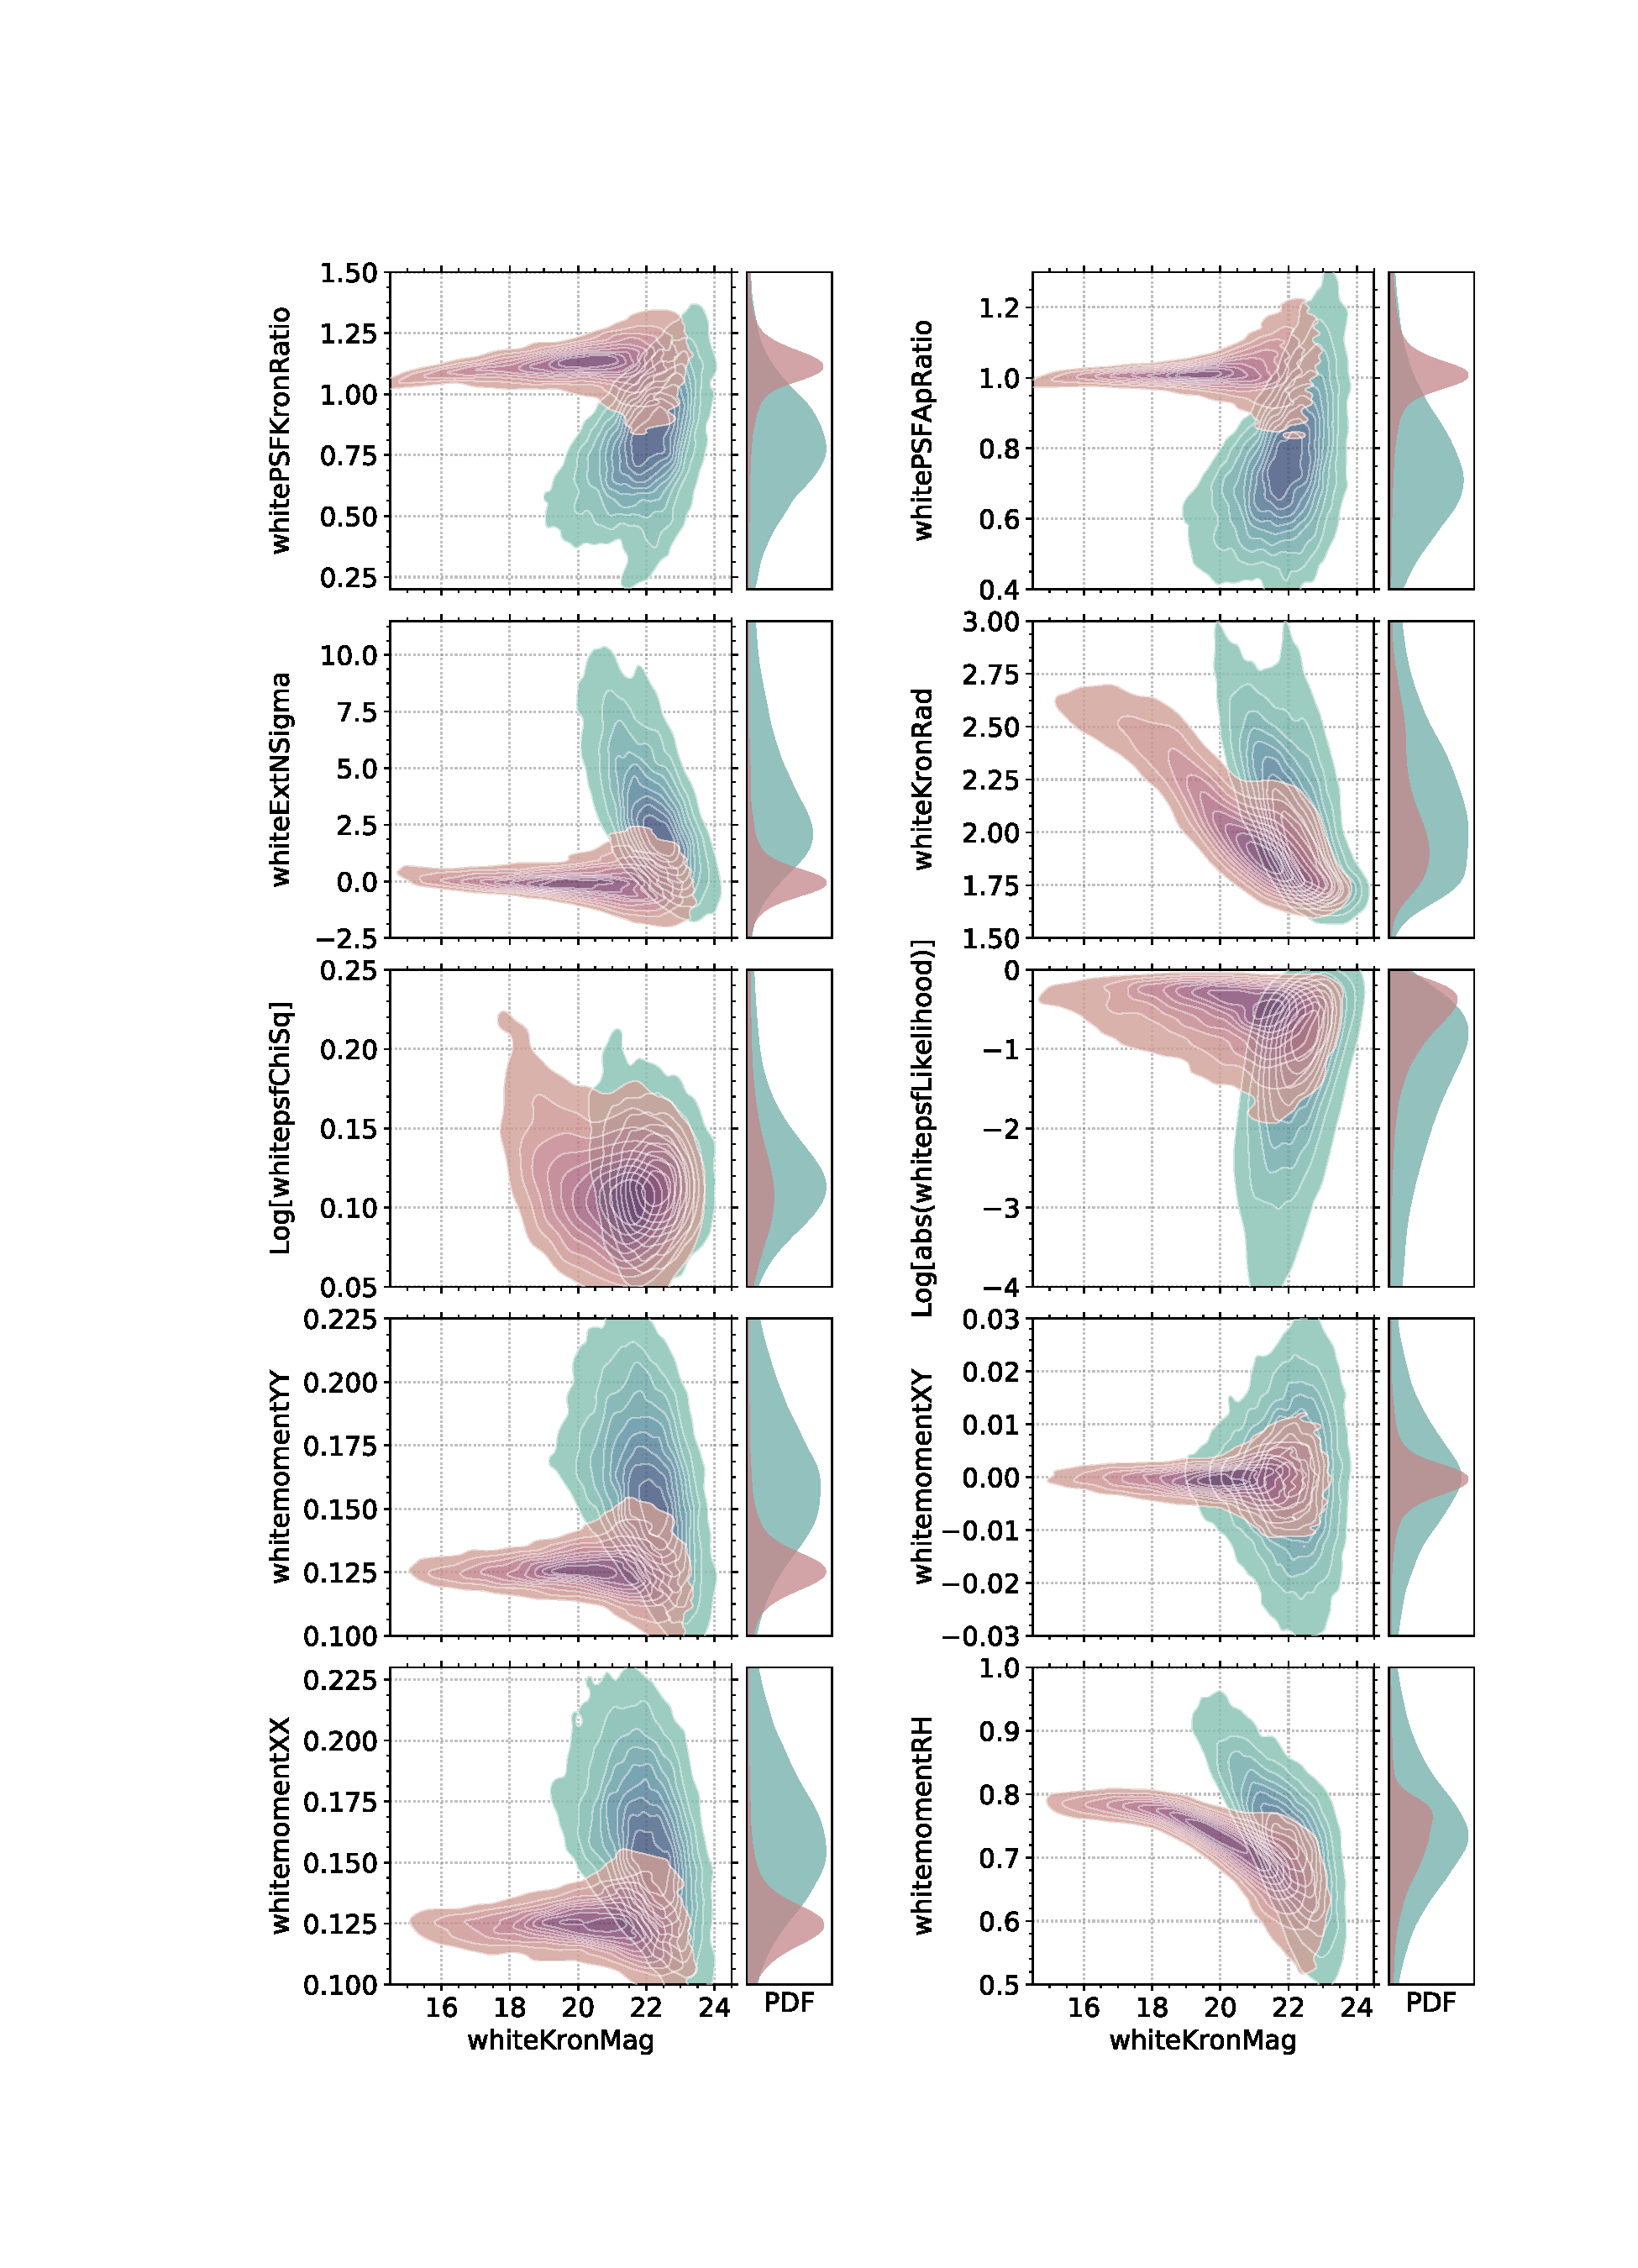
\includegraphics[width=5.75in
  %,bb = 0 0 864 1296
  ]{./Figures/whiteFeatures.pdf}
  \caption{
  The primary square panels show KDEs of the PDF for each of the ``white
  flux'' features as a function of \texttt{whiteKronMag}
  ($=-2.5\log_{10}[\mathtt{whiteKronFlux}/3631]$) for all sources in the
  \textit{HST} training set. Stars are shown via the red-purple contours,
  while galaxies are shown via blue-green contours. The shown contour levels
  extend from 0.9 to 0.1 in 0.1 intervals. To the right of each primary panel
  is a marginalized 1D KDE of the PDF for the individual features, where the
  amplitudes of the KDEs have been normalized by the relative number of stars
  and galaxies. The clear overlap between faint stars and galaxies suggests
  that a machine learning model may provide significant improvement over the
  PS1 and simple models.}
  %
  \label{fig:features}
\end{figure*}

The distribution of ``white flux'' features for stars and galaxies in the
\textit{HST} training set is shown in Figure~\ref{fig:features}
(\texttt{whitePSFKronDist} is shown in Figure~\ref{fig:psfkrondist}). As
might be expected, it is clear from Figure~\ref{fig:features} that stars and
galaxies are easily separated at the bright end ($\lesssim 20$\,mag), but
there is significant overlap in the featurespace between the two populations
at the faint end ($\sim$23\,mag). Machine learning algorithms are capable of
capturing non-linear behavior in multidimentional data sets, which will
prove especially useful for the sources under consideration in the PS1 data
set.

\section{Model Construction}
\subsection{The PS1 Baseline Model}\label{sec:ps1_model}

To establish a baseline for the performance of our star-galaxy separation
models we adopt the classification criteria in the PS1 documentation, namely
sources with 
%
$$ \mathtt{iPSFMag} - \mathtt{iKronMag} > 0.05\;\mathrm{mag},$$
%
are classified as
galaxies.\footnote{\url{https://outerspace.stsci.edu/display/PANSTARRS/How+to+
separate+stars+and+galaxies}} The documentation notes that this
classification can be performed using photometry from any of the
\textit{MeanObject}, \textit{ForcedMeanObject}, or \textit{StackedObjectThin}
tables. The PS1 documentation further notes that this basic cut does not
perform well for sources with $i \gtrsim 21\,\mathrm{mag}$, which constitutes
the majority of sources detected by PS1, and motivates us to develop
alternative models. We use the performance of the $\mathtt{iPSFMag} -
\mathtt{iKronMag} > 0.05\;\mathrm{mag}$ model (hereafter, the PS1 model) as a
baseline to compare to the models discussed below.

\subsection{Simple Model}\label{sec:simple_model}

While our ultimate goal is to build a machine learning model to separate
stars and galaxies (\S\ref{sec:rf_model}), we first construct a
straightforward model. This model is inspired by the SDSS \texttt{photo}
pipeline \citep{Lupton01}, and combines the flux in each of the 5 PS1 filters
to improve the SNR relative to any individual band. In addition to being easy
to interpret, this model (hereafter, the simple model), which utilizes the
difference between the PSF flux and the Kron-aperture flux for
classification, serves as an additional baseline to test the need for a more
complicated machine learning model.

It stands to reason that a model built on all five PS1 filters should outperform a model constructed from a single filter. To that end, we examine the \texttt{whitePSFKronRatio} (equivalent to $\mathtt{whitePSFMag} - \mathtt{whiteKronMag}$) to discriminate between stars and galaxies. The upper left panel of Figure~\ref{fig:features} shows that sources with $\mathtt{whitePSFKronRatio} \gtrsim 1$ are very likely to be stars. A single hard cut on \texttt{whitePSFKronRatio}, similar to the SDSS \texttt{photo} pipeline or the PS1 model, removes any sense of confidence in the corresponding classification. For example, a source with $\mathtt{whitePSFKronRatio} = 1.1$ and $\mathtt{whiteKronMag} \approx 17\,\mathrm{mag}$ is far more likely to be a star than a source with the same \texttt{whitePSFKronRatio} value but $\mathtt{whiteKronMag} \approx 23\,\mathrm{mag}$ (see Figure~\ref{fig:features}).

To address this issue of classification confidence, we measure the
orthogonal distance from a line ($\mathtt{whitePSFFlux} = a\times
\mathtt{whiteKronFlux}$) for all sources in the
$\mathtt{whitePSFFlux}$--$\mathtt{whiteKronFlux}$ plane to define the simple model:
%
\begin{multline}
 \mathtt{whitePSFKronDist}(a) = \\
 \frac{\mathtt{whitePSFFlux} - a\times\mathtt{whiteKronFlux}}{ \sqrt{1 + a^2}},
 \label{eqn:psfkrondist}
\end{multline}
%
where $a$ is the slope of the line. For $a \approx 1$, which is similar to a
hard cut with $\mathtt{whitePSFKronRatio} = a$, bright stars will have
large, positive values of \texttt{whitePSFKronDist}, while bright galaxies
will have large, negative values of \texttt{whitePSFKronDist}.
Simultaneously, faint sources, which are more difficult to classify, will
have small values of \texttt{whitePSFKronDist}. The simple model allows us
to produce a rank ordered classification, which in turn allows us to
evaluate the optimal classification threshold for the separation of stars
and galaxies (see \S\ref{sec:comp_hst}).

The optimal value for $a$ is determined via $k$-fold cross validation (CV).
We adopt identical procedures to optimize both the simple model and the
machine learning model (see \S\ref{sec:rf_model}). We employ the use of an
inner and outter CV loop, both of which have $k = 10$ folds. In the outter
CV loop, the training set is split into 10 separate partitions, each
iteratively withheld from the training. For each partition in the outter CV
loop, an inner 10-fold CV is applied to the remaining $\sim$90\% of the
training set to determine the optimal model parameters. Predictions on the
sources withheld in the outter loop are made with the optimal model from the
inner loop to provide model predictions for every source in the training
set. We adopt final, optimal tuning parameters from the mean of the values
determined in the inner CV.

For the simple model, we employ a grid search over $a$ in the inner CV loops
to maximize the FoM and thereby determine the optimal value of $a$.
Initially, a wide grid from 0 to 2 was searched, followed by a fine grid
search over $a$ from 0.75 to 1.25 with step size = 0.0025. The average
optimal $a$ from the inner loops, and hence final model value, is 0.91375,
with sample standard deviation $\sim$0.01. From this procedure, we find that
for the simple model the $\mathrm{FoM} = 0.62 \pm 0.02$, where the
uncertainty is estimated from the scatter in the outter CV
results.\footnote{We find that PS1 flux measurements from the
\textit{StackObjectThin} table produce a higher FoM for the simple model
than flux measurements from the \textit{MeanObject} and
\textit{ForcedMeanObject} tables. Thus, we adopt \textit{StackObjectThin}
fluxes for both the simple model and the machine learning model, as noted in
\S\ref{sec:model_data}.}


\begin{figure}[t]
 \centering
  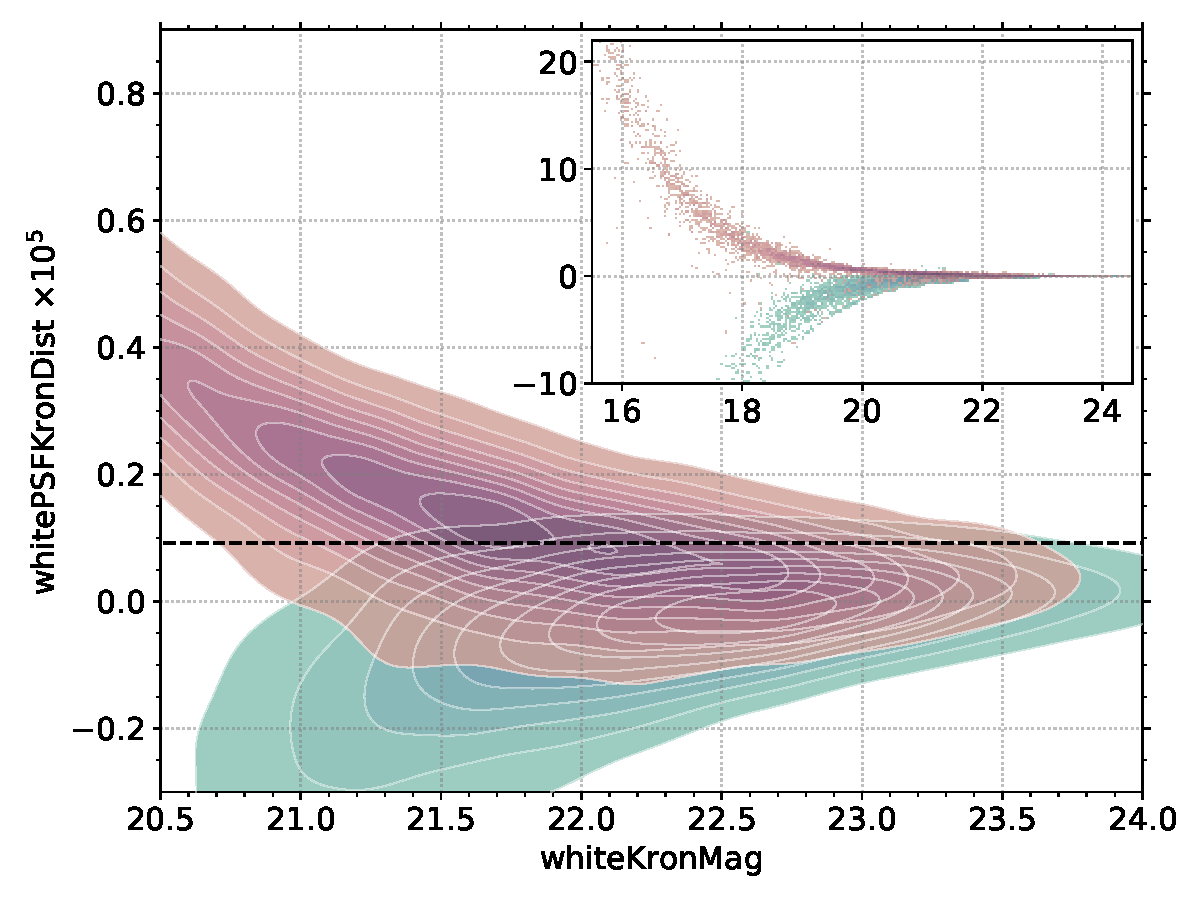
\includegraphics[width=3.55in
  %,bb = 0 0 576 432
  ]{./Figures/whitePSFKronDist.pdf}
  %
  \caption{ The distribution of $\mathtt{whitePSFKronDist}$ values for
  \textit{HST} training set stars and galaxies as a function of
  \texttt{whiteKronMag}. The colors and contours are the same as
  Figure~\ref{fig:features}. The horizontal dashed line shows the optimal
  threshold ($\mathtt{whitePSFKronDist} \ge 9.2 \times 10^{-7}$) for
  star--galaxy classification. The upper-right inset shows a zoom-out
  highlighting the stark difference between stars and galaxies at the bright
  end. }
  %
  \label{fig:psfkrondist}
\end{figure}

The distribution of $\mathtt{whitePSFKronDist}(a=0.91375)$ is shown for
\textit{HST} training set stars and galaxies in
Figure~\ref{fig:psfkrondist}. $\mathtt{whitePSFKronDist}$ provides an
excellent discriminant between bright ($\lesssim 20\,\mathrm{mag}$) stars
and galaxies. We further find that adopting a stellar classification
threshold of $\mathtt{whitePSFKronDist} \ge 9.2 \times 10^{-7}$ produces a
classification accuracy of $\sim$91\%.

\subsection{Random Forest Model}\label{sec:rf_model}

\subsubsection{The Random Forest Algorithm}\label{sec:rf_alg}

Based on its success in previous astronomical applications (e.g., \citealt{Richards12a, Huppenkothen17, Brink13, Wright15, Goldstein15}), including
star--galaxy separation (e.g., \citealt{Vasconcellos11,Miller17}), we adopt
the RF algorithm \citep{Breiman01} for our machine learning model. Briefly,
RF is built on decision tree models \citep{Quinlan93} that utilize bagging
\citep{Breiman96}, wherein bootstrap samples of the training set are used to
train each of the $N_{\mathrm{tree}}$ individual trees. Within the
individual trees, only $m_{\mathrm{try}}$ randomly selected features are
used to separate sources at each node, and nodes cannot be further split if
there are fewer than \texttt{nodesize} sources in the node. The randomness
introduced by both bagging and the use of $m_{\mathrm{try}}$ features
reduces the variance of RF predicitions relative to single decision tree
models. Final RF classifications are determined via a majority vote from
each of the $N_{\mathrm{tree}}$ individual trees. Thus, RF models are
capable of producing low-variance, low-bias predictions. We utilize the
\texttt{Python scikit-learn} implementation of the RF algorithm
\citep{Pedregosa12} in this study.

\subsubsection{Feature Selection}

While the RF algorithm is relatively insensitive to correlated and/or weak/uninformative features (e.g., \citealt{Richards12a}), we nevertheless investigate if removing features from our feature set improves the model performance.\footnote{For example, we find a strong correlation between \texttt{whiteExtNSigma} and \texttt{whitepsfLikelihood}, $r = 0.846448$, which may harm the final model classification. \yutaro{Is this the Pearson correlation coefficient? We should give an exact number here. : Y
es, this value is the Pearson correlation coefficient. 
I had forgotten removing sources with \texttt{nDetections=0} in the previous version, 
so the value is changed slightly.}}
 We do this via forward and backward feature selection (\yutaro{there is a good reference for this - check my 2015 paper if you haven't read it: I read it. Thank you!}). Forward and backward feature selection involve the iterative addition or removal of features from the model, respectively. Like \citet{Richards12a}, we rank order the features for either addition or subtraction based on their RF-determined importance \citep{Breiman02}.
In either case, we find that removing features does not improve the CV FoM, and therefore include all 11 features from \S\ref{sec:model_features} the final RF model.

\subsubsection{Optimizing the Model Tuning Parameters}

As noted in \S\ref{sec:simple_model}, we optimize the RF model tuning parameters via an outter and inner 10-fold CV procedure. We perform a grid search over $N_{\mathrm{tree}}$, $m_{\mathrm{try}}$ and \texttt{nodesize}, and find that the FoM of \textit{HST} training is maximized with $N_{\mathrm{tree}} = 400$, $m_{\mathrm{try}} = 4$, and $\mathtt{nodesize} = 2$. The final model FoM is not strongly sensitive to the choice of these parameters: changing any of the optimal parameters by a factor of $\sim$2 does not decrease the optimal CV FoM, 0.72, by more than the scatter measured from the individual folds, 0.02. Finally, while a detailed comparison is presented in \S\ref{sec:comp_hst}, we note that the RF model significantly outperforms the simple model based on the CV FoM.

\todo{check why FoM does not match Table 1}

\section{Classification Performance}

\subsection{PS1, Simple, and RF Model Comparison}\label{sec:comp_hst}

We assess the relative performance of the RF model by comparing it to both
the PS1 and simple models. To do so, we select the subset of sources from
the \textit{HST} training set that have $\mathrm{det}_{i_\mathrm{PS1}} = 1$
(the PS1 model cannot classify sources that are not detected in the
$i_\mathrm{PS1}$ band), which results in 40,098 sources.

Figure~\ref{fig:cvroc_hst} shows that the RF model and simple model provide
substantial improvements over the PS1 model, with $\sim$10,000\% and
$\sim$9,200\% respective increases in the FoM relative to the PS1 model.
\yutaro{check these numbers after checking ROC procedure} We additionally
show Receiver Operating Characteristic (ROC) curves for the 3 models in
Figure~\ref{fig:cvroc_hst}. ROC curves show how the true positive rate
(TPR)\footnote{$\mathrm{TPR} = \mathrm{TP}/(\mathrm{TP} + \mathrm{FP})$,
where TP is the total number of true positive classifications and FP is the
number of false positives.} and false positive rate
(FPR)\footnote{$\mathrm{FPR} = \mathrm{FP}/(\mathrm{FP} + \mathrm{TN})$,
where TN is the number of true negatives.} vary as a function of
classification threshold. As a reminder, stars are considered the positive
class in this study. To construct ROC curves for the simple and PS1 models
we vary the classification thresholds from $\mathrm{whitePSFKronDist} =
\yutaro{4.24524\times 10^{-3}}$ to \yutaro{$-16.23348\times10^{-3}$} and
$\mathtt{iPSFMag} - \mathtt{iKronMag} =
\yutaro{5.09913363}\;\mathrm{mag}$ to
$\yutaro{-2.81103881}\;\mathrm{mag}$, respectively.
Figure~\ref{fig:cvroc_hst} highlights the strength of the simple model
approach: by using a metric that essentially captures both the difference
between the PSF and Kron-aperture measurements \textit{and} the SNR, the
simple model produces much higher TPR at low FPR than the PS1 model, which
eliminates any information about the SNR.

Summary statistics showing the superior performance of the RF model relative
to the simple and PS1 models are presented in Table~\ref{table:hst_cv}.
These statistics include the FoM, the integrated area under the ROC curve
(ROC AUC), and the overall accuracy of the 3 models as evaluted on the
subset of \textit{HST} training set sources with $i_\mathrm{PS1}$
detections. We use 10-fold CV to measure the summary statistics, with
identical folds for each model. Strictly speaking, this CV procedure is only
needed for the RF model, which needs to be re-trained for every fold, but
testing the simple and PS1 models on the individual folds provides an
estimate in the scatter of the final reported metrics. From
Table~\ref{table:hst_cv} it is clear that the RF model greatly outperforms
the simple and PS1 models.


\begin{deluxetable}{cccc}
    \tablecolumns{4} 
    \tablewidth{0pt} 
    \tablecaption{ CV Results for \textit{HST} Training Set \label{table:hst_cv}}
    \tablehead{ 
    \colhead{model} & \colhead{FoM} & \colhead{Accuracy} & \colhead{ROC AUC}
    }
    \startdata
    RF & \textbf{0.708} $\pm$ 0.037 & \textbf{0.932} $\pm$ 0.003 & \textbf{0.973} $\pm$ 0.002 \\
    simple & 0.657 $\pm$ 0.020 & 0.916 $\pm$ 0.003 & 0.937 $\pm$ 0.004 \\
    PS1 & 0.007 $\pm$ 0.003 & 0.784 $\pm$ 0.006 & 0.851 $\pm$ 0.006 \\
    \enddata
\end{deluxetable}

%%% fig:cvroc_hst %%%
\begin{figure}[t]
 \centering
  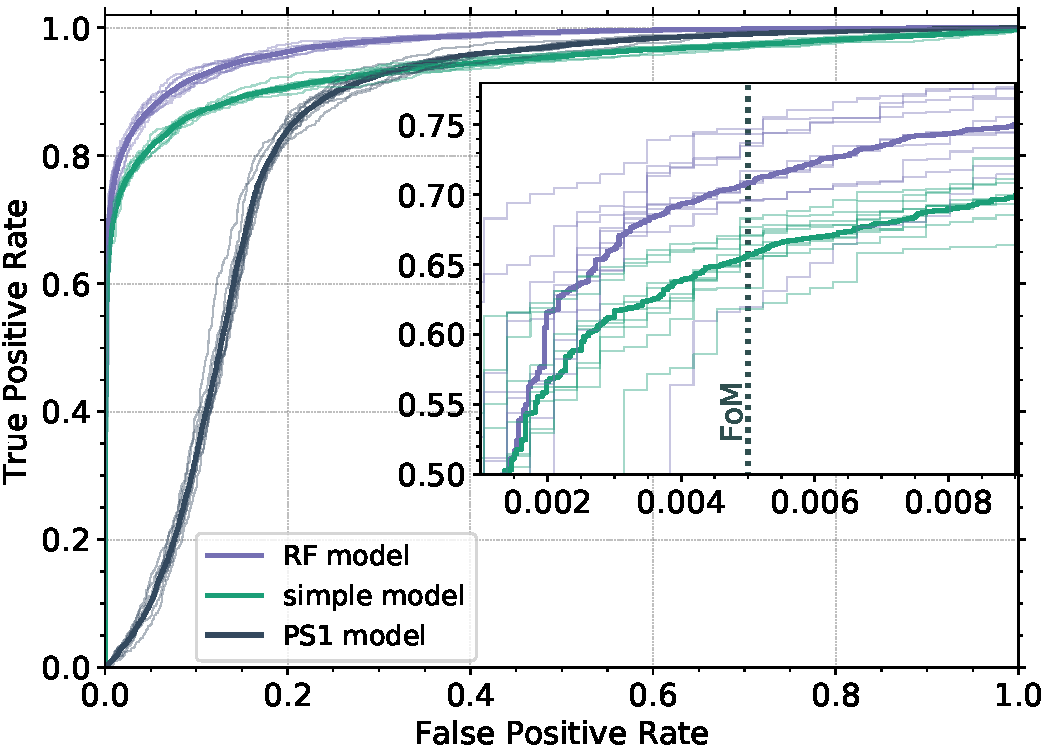
\includegraphics[width=3.35in
  %,bb = 0 0 504 360
  ]{./Figures/CV_ROC_HST.pdf}
  %
  \caption{ ROC curves comparing the relative performance of the PS1,
  simple, and RF models as tested by the subset of \textit{HST} training set
  sources with $i_\mathrm{PS1}$ detections. The thick, solid orange, blue,
  and black lines show the ROC curves for the PS1, simple, and RF models,
  respectively. The light, shaded regions bounding these lines show the
  10-fold CV scatter about the mean model. The inset on the right shows a
  zoom in around FPR = 0.005, shown as a vertical line, corresponding to the
  FoM (the PS1 model is not shown in the inset, because it has very low
  FoM). }
  %
  \label{fig:cvroc_hst}
\end{figure}
%%%%%%%%%%%%%

% Since the ML model is trained with the 11 features
% consisting \texttt{whitepsfKronDist} and \texttt{whitepsfKronRatio},
% which is the fundamental information for the classification in the  simple model and the PS1 model, respectively,
% the TPR of the ML model is higher than that of baseline models in whole FPR value.
% The ROC AUC is 0.973, 0.937, and 0.851,
% and the FoM is 0.715, 0.658, and 0.007,
% for the PS1 model, the simple model, and the ML model, respectively;
% in the other words, the TPR at the FPR$=0.5\%$ of the ML model and the simple model
% is improved 70.8$\%$ and 65.1$\%$ from that of the PS1 model, respectively.
% The overall CV accuracy of the ML model, the simple model, and the PS1 model is
% 93.3\%, 91.6\%, and 78.4\%.

%%% fig:cvacc_hst %%%
\begin{figure}[t]
 \centering
  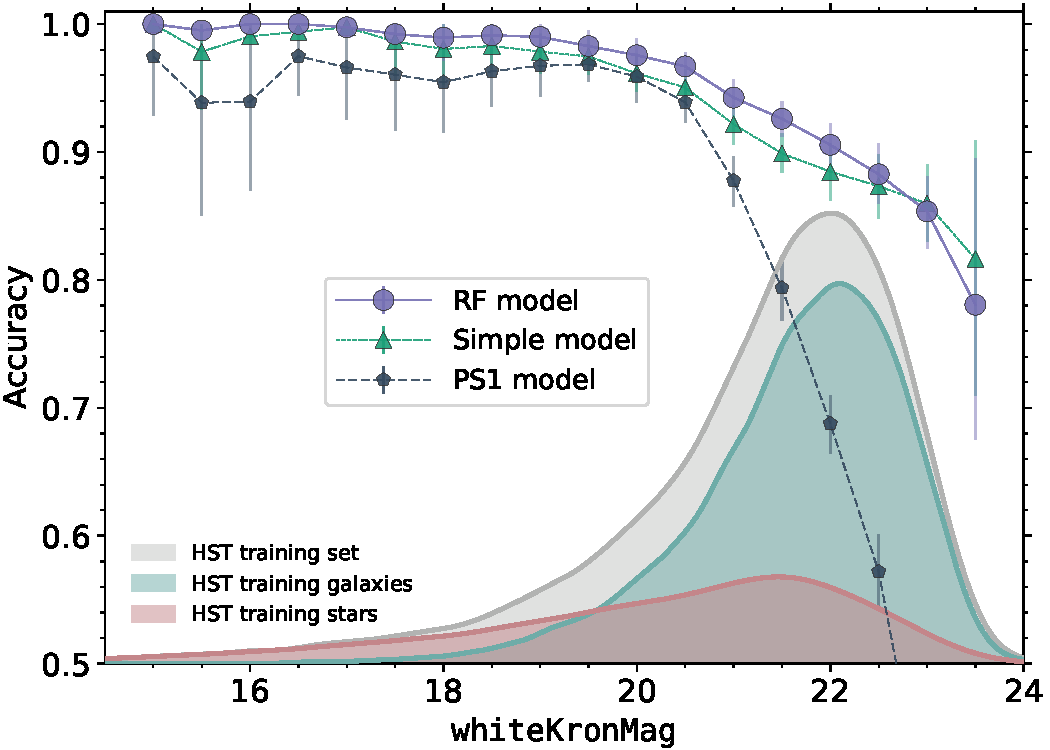
\includegraphics[width=3.5in
  %,bb = 0 0 576 360
  ]{./Figures/CV_Accuracy_HST.pdf}
  %
  \caption{Model accuracy as a function of \texttt{whiteKronMag} evaluated
  on the subset of the \textit{HST} training set sources with
  $i_\mathrm{PS1}$ detections. Accuracy curves for the PS1, simple and RF
  models are shown in orange, blue, and black, respectively. The bin widths
  are 0.5\,mag, and the error bars represent the range including 68\% of CV
  accuracies in each bin. \yutaro{I think we should use bootstrap for
  uncertainties} Additionally, a Gaussian KDE of the PDF for the entire
  \textit{HST} training set subset, as well as the stars and galaxies in the
  subset is shown in the shaded grey, red, and green regions, respectively.
  The amplitude of the star and galaxy PDFs have been normalized by their
  relative ratio compared to the full subset. }
  %
  \label{fig:cvacc_hst}
\end{figure}
%%%%%%%%%%%%%

The classification accuracy for each model as a function of
\texttt{whiteKronMag} is shown in 0.5\,mag bins in
Figure~\ref{fig:cvacc_hst}. The accuracies are estimated via 10-fold CV (see
above) and the uncertainties represent the inter-68\% interval from
\yutaro{CCC} bootstrap samples within each bin. \yutaro{Is this correct?}
The classification thresholds for the RF, simple, and PS1 models are 0.5,
$9.2 \times 10^{-7}$, and 0.05, respectively. Again, the RF and simple
models provide a significant improvement over the PS1 model. The PS1 model
provides classification accuracies $\gtrsim$90\% for sources with
$\mathtt{whiteKronMag} \lesssim 21\,\mathrm{mag}$, but precipitously
declines for fainter sources. The RF and simple models have similar curves
with the RF model performing slightly better, as is to be expected given
that the RF model uses 10 additional features beyond
\texttt{whitePSFKronDist}.

\subsection{Model Evaluation via an Independent Test Set}

%%% fig:roc_sdss %%%
\begin{figure}[t]
 \centering
  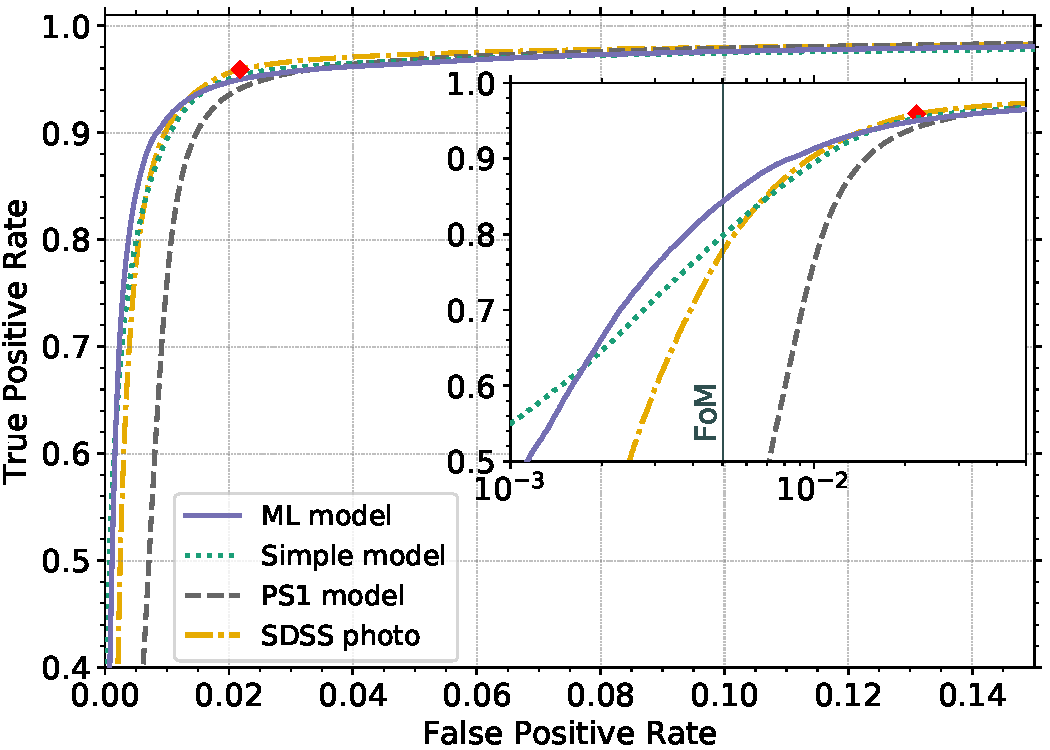
\includegraphics[width=3.35in
  %,bb = 0 0 576 360
  ]{./Figures/ROC_curves.pdf}
  \caption{
  ROC curves comparing the relative performance 
  of the SDSS photo model (green solid line), the PS1 model (orange solid line), 
  the simple model (blue solid line), and the Ml model (black solid line) 
  for PS1 sources cross-matched against the SDSS spectroscopic catalog. 
  The SDSS photometric classifier is shown as a red star on the ROC curve of the SDSS photo model, 
  due to the binary nature of the SDSS photometric classification. 
  The inset panel shows ROC curves around the FPR = 0.005 (grey solid line). 
  }
  %
  \label{fig:roc_sdss}
\end{figure}
%%%%%%%%%%%%%

While CV on the \textit{HST} training set shows that the RF models
outperforms the alternatives, here, we test each of the previous models with
the SDSS training set, which provides an independent set of $\sim$3.5$\times
10^6$ (\NC{3,834,627?}) sources with high-confidence labels. Additionally, the use of SDSS
spectra allows us to compare our new models to the classifications from the
SDSS \texttt{photo} pipeline, hereafter the SDSS model, which soundly
outperformed the PTF RF star--galaxy models \citep{Miller17}. We create an
ROC curve for the SDSS model by thresholding on the ratio of PSF flux to
\texttt{cmodel} measured in the SDSS images (see \citealt{Miller17} for more
details).

To compare the 4 models, we select the subset of SDSS training set sources
that have $i_\mathrm{PS1}$ detections (to compare with the PS1 model) and
SDSS \texttt{photo} classifications (to compare with the SDSS model), and
show ROC curves for each model applied to this subset of sources
(\NC{3,592,940} total \NC{we also excluded QSOs with $z<1$ and galaxies 
with $z<10^{-4}$ from the SDSS training set}) 
in Figure~\ref{fig:roc_sdss}. The FoM for the PS1,
simple, and RF models is higher as tested by SDSS spectroscopic sources
because the SDSS training set contains brighter, higher SNR (and hence
easier to classify) sources. As before, we find that the FoM for the RF
model is superior to the alternatives. Interestingly, we also find that the
ROC curves cross, and that the SDSS model provides the largest TPR for
$\mathrm{FPR} \gtrsim 0.015$. That the RF and SDSS curves cross suggests
that there may be regimes where the SDSS \texttt{photo} classifications are
superior to the RF model. Below, we argue that a bias in the SDSS training
set is amplified by a bias in the SDSS \texttt{photo} classification, which
is why these curves cross.

% Although the data set has the selection bias as mentioned above and thus the
% distribution of stars and galaxies as a function of brightness is totally
% different to that of the training set, the ROC curve of ML model is superior
% to the other models in terms of the FoM and also the ROC AUC; the FoM for
% the SDSS model, the PS1 model, the simple model, and the ML model is 0.777,
% 0.290, 0.798, and 0.843, respectively, and the ROC AUC score for each model
% is 0.987, 0.984, 0.985, and 0.987, respectively.

% Next, we assess the performance of the ML model by comparing with SDSS photometric classification
% by using PS1-SDSS spectroscopic catalog.
% Figure \ref{fig:roc_sdss} shows the ROC curve for
% the SDSS photo, the PS1 model, the simple model, and the ML model,
% by comparing predictions with SDSS spectroscopic classifications,
% which are independent of the training data set; PS1-HST cross-matched catalog.
% For sources in PS1-SDSS catalog, broadly,
% the performance of classifications by each model is better than that for sources in PS1-HST catalog.
% This is simply because that the distribution of sources, especially galaxies, in PS1-SDSS catalog
% are biased toward to brighter side comparing with of PS1-HST catalog.
% The selection bias of the SDSS spectroscopic survey
% toward observing luminous red galaxies (LRGs; {\it e.g.,} see \citealt{Eisenstein01})
% results in the KDE of the PDF of galaxies having two peaks
% at $\mathtt{whiteKronMag} \sim 17$ and $\sim 20$
% (see \S\ref{sec:sdss} and the left panel in Figure \ref{fig:acc_sdss}).
% As we alluded to in \S\ref{sec:comp_hst},
% the distribution of stars and galaxies in the real universe (except the galactic plane)
% should be similar to that shown in Figure \ref{fig:cvacc_hst};
% the peak of the distribution for stars and galaxies is around $\mathtt{whiteKronMag} \sim 22$
% and the number of stars and of galaxies is dominant at the bright end and the faint end,
% respectively \citep{Chambers16}.

%%% fig:acc_sdss %%%
\begin{figure*}[t]
 \centering
  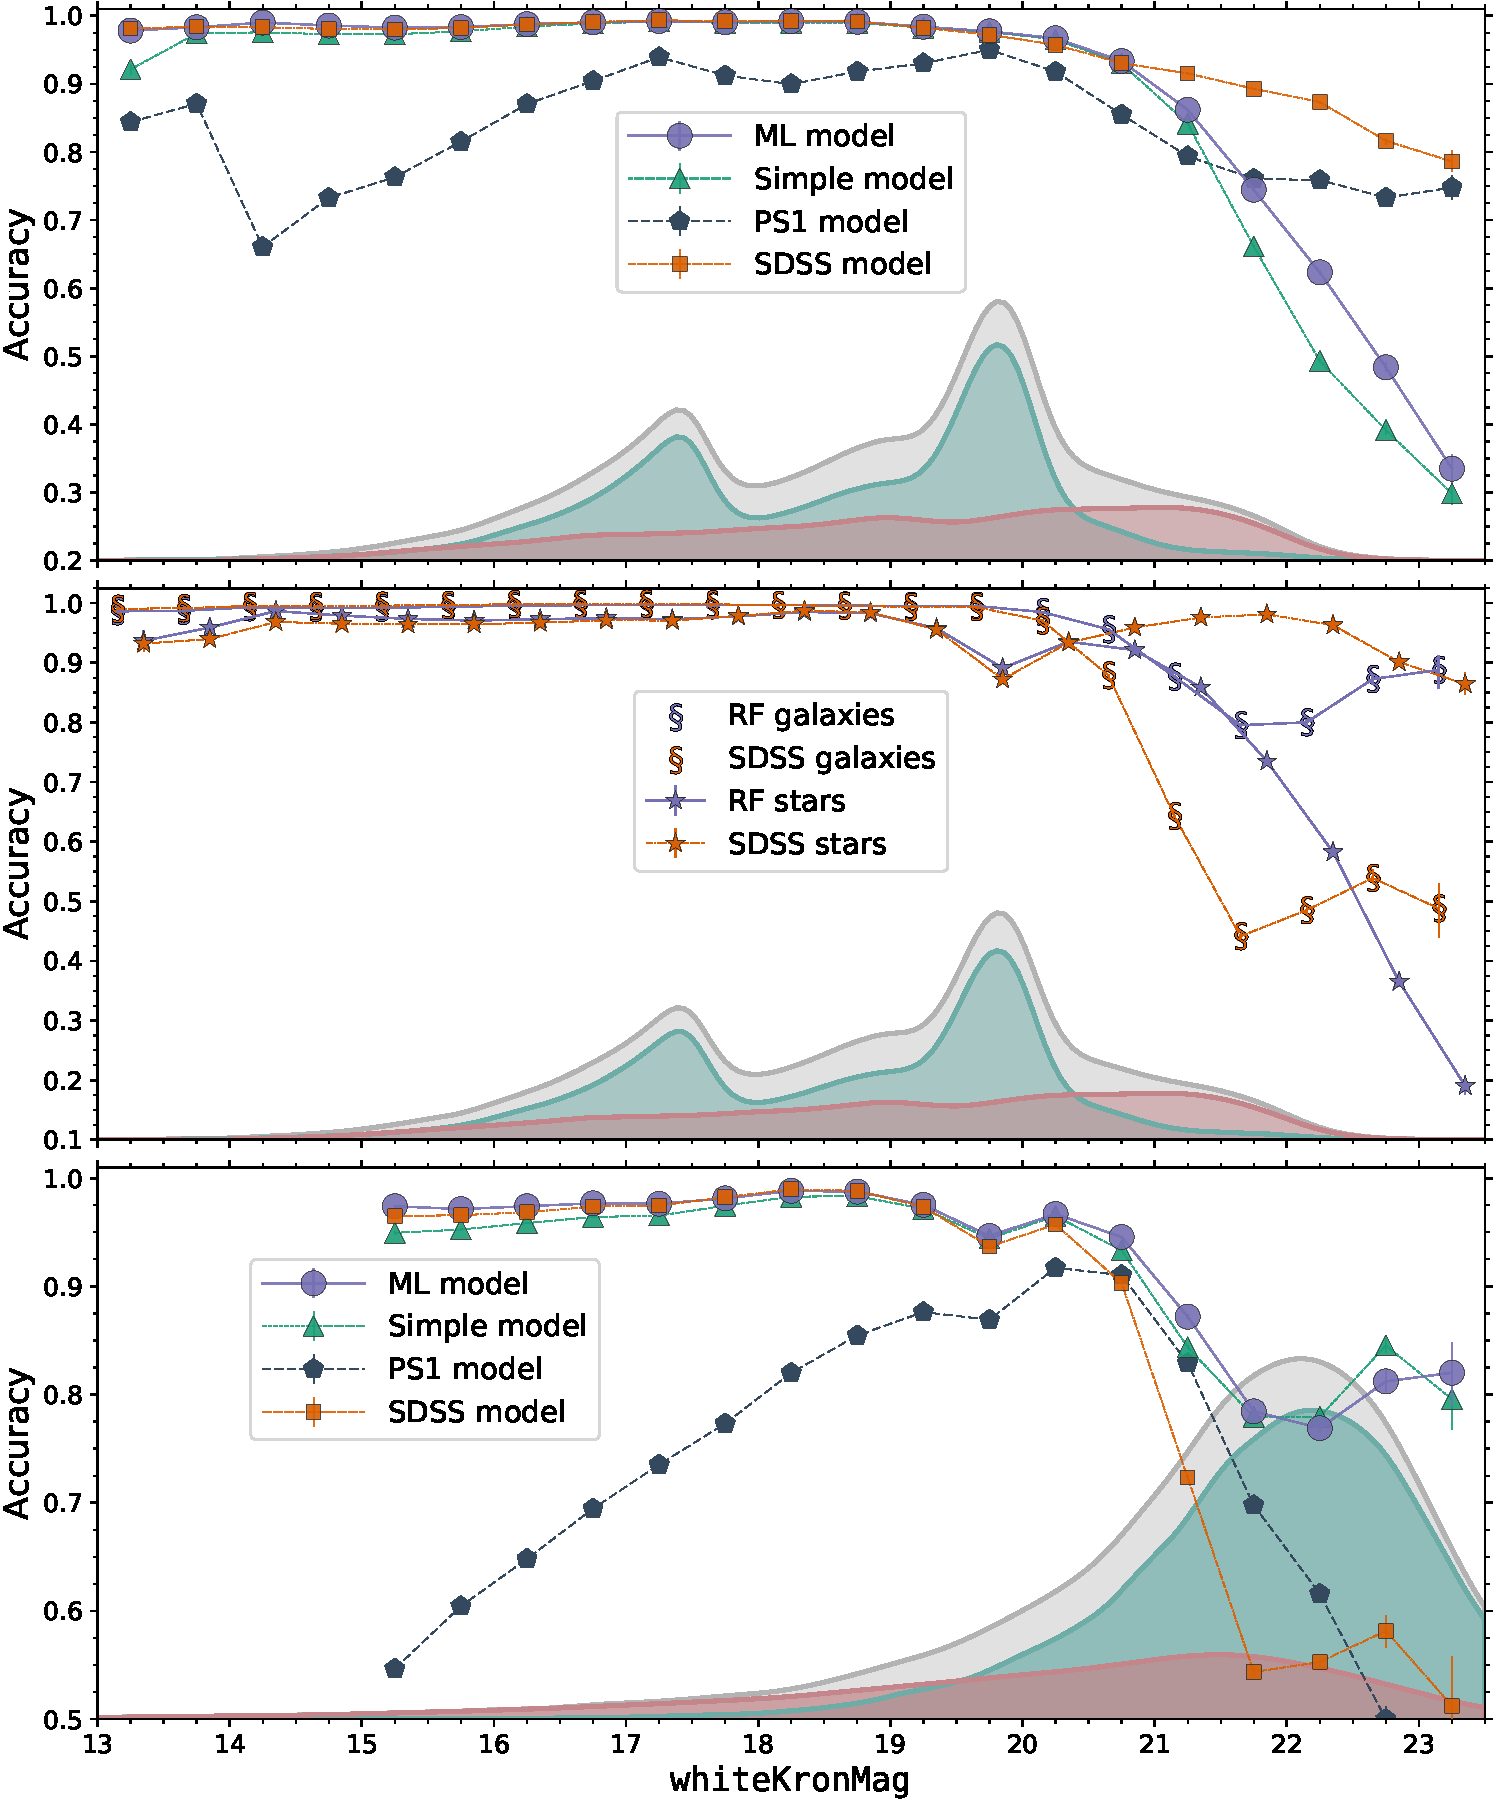
\includegraphics[width=6.5in
  %,bb = 0 0 576 864
  ]{./Figures/SDSS_acc_mag.pdf}
  \caption{
  Prediction accuracy of the SDSS photo model and the ML model 
  as a function of \texttt{whiteKronmag} for PS1 sources cross-matched against the SDSS spectroscopic catalog. 
  In the left panel, the green filled square and the green filled triangle 
  show the prediction accuracy of the SDSS photo model for galaxies and stars, respectively, 
  and the black filled square and the black filled triangle show that of the ML model for galaxies and stars, respectively. 
  Accuracies are calculated in each 0.5 mag bin. 
  The KDE of the normalized PDF of stars and galaxies 
  in the PS1-SDSS cross-matched catalog is also shown in red and green, respectively (same manner as Fig. \ref{fig:cvacc_hst}). 
  In the right panel, the overall accuracy of the SDSS photo model and the ML model 
  as a function of \texttt{whiteKronMag} is shown by filled green circle and filled black circle, respectively. 
  The accuracy in each bin is calculated for stars and galaxies picked up 
  from PS1-SDSS cross-matched catalog 
  so that the ratio the number of stars and galaxies in each bin is 
  same with that in the PS1-HST cross-matched catalog. 
  The KDE of PDF of stars and galaxies in PS1-HST cross-matched catalog is shown in red and green, respectively. 
  } 
  %
  \label{fig:acc_sdss}
\end{figure*}
%%%%%%%%%%%%%


\NC{In the left panel of Figure \ref{fig:roc_sdss}, we show the prediction accuracy of the SDSS photo model 
and the ML model for galaxies and stars separately. 
One can see that an unusual systematic whereby a large fraction of stars with $\mathtt{whiteKronMag} \sim 20$ 
were erroneously classified as galaxies by both of models. 
The reason of it is discussed by \cite{Miller17}; 
red stars blended with fainter sources would be classified to be galaxies. 
Interestingly, for the SDSS photo model, the accuracy for galaxies is rapidly decreasing from \texttt{whiteKronMag}, 
while that for stars stays above $\sim 0.9$. 
It means the SDSS photo model is optimized to separate stars and galaxies in the SDSS spectroscopic catalog, 
namely, the model classifies most of faint sources as stars 
since the number of stars overwhelms that of galaxies from $\sim 21$ mag to the faint end in this catalog. 

For evaluating the performance of the SDSS photo model and the ML model 
for the star/galaxy population similar to the real universe, 
we calculate the prediction accuracy of each model in a different way; 
we pick up sources from PS1-SDSS catalog 
so that the ratio of the number of stars and to the number of galaxies 
is same as that in PS1-HST catalog, and then calculate the prediction accuracy of each model in each 0.5 mag bin. 
The result is shown in the right panel of Figure \ref{fig:acc_sdss}. 
The prediction accuracies shows that the performance of each model is similar 
down to $\mathtt{whiteKronMag} \sim20.5$, 
while the performance of the SDSS photo model quickly degrades for fainter sources. 
This is to be expected based on the poor performance for faint galaxies of the SDSS photo model; 
the PS1-HST catalog (and also the real universe) contains much larger number of faint galaxies than faint stars. 
The final ML model, which is optimized to classify stars and galaxies following this population, 
will provide the most accurate classification for sources in high-latitude sky. 
} 

% \section{Discussion}

\section{The PS1 Catalog Deployed: Integration in ZTF}

\todo{provide a description for how the catalog is used by ZTF in real-time ops}

The Zwicky Transient Facility (ZTF; 
\citealt{Kulkarni12, Bellm14, Smith14, Dekany16, Bellm17})\footnote{\url{http://www.ztf.caltech.edu/}} 
was started and had the first light at Palomar Observatory in 2017, 
as the next generation Palomar time-domain survey 
subsequent to the Palomar Transient Facility (PTF; \citealt{Rau09, Law09}) 
and the intermediate Palomar Transient Facility (iPTF; \citealt{Kulkarni13}). 
A dedicated survey of the variable sky by ZTF is ongoing with the new camera 
utilizing the entire focal plane on 47 deg$^2$ of the Palomar 48-inch Samuel Oschin Schmidt telescope. 
ZTF is scanning more than 3,750 deg$^2$ an hour to depth $R < 20.4$ mag ($5\sigma$ detection), 
and will produce a photometric variability catalog with nearly 300 observations each year. 
A primary motivation for ZTF is the search for fast transients 
including ``kilonovae'' 
associated with gravitational waves, 
the result of binary neutron star mergers 
(GW170817; {\it e.g.,} \citealt{Abbott17, Cowperthwaite17, Lipunov17, Kasliwal17, Utsumi17, Tanaka17}). 

ZTF surveys the sky at a rate that is $\sim15$ times faster than PTF/iPTF. 
The increase in the amount of astronomical data with a rapidly accelerating pace 
results in the necessity of automated classification and filtering by machines to investigate objects 
that we are potentially interested in. 
To identify fast-transient candidates, including gravitational wave (GW) counterparts especially, 
astronomers have contended with significant foreground contamination in the form of stellar flares 
and/or orbital modulation ({\it e.g.,} \citealt{Kulkarni06, Berger12, Kasliwal16}). 
The systematic removal of faint stars from extragalactic candidate lists 
enables us to follow-up such exotic sources efficiently under the limitation of time, instrumental, and human resources. 
The follow-up efficiency will be required more strongly from the beginning of the third observing run of LIGO/VIRGO 
collaborating with KAGRA in 2019. 


\section{Conclusions}

%%%%%%%%
\begin{table*}
\begin{center}
\caption{The true positive ratio and the threshold 
corresponding to the false positive ratio = 0.005, 0.01, 0.02, 0.05, and 0.1. }
\label{tbl:fpr}
\begin{tabular}{lcc|lccccc}
\hline\hline
                 Source               & Num. & Acc. & FPR & 0.005 & 0.01 & 0.02 & 0.05 & 0.1 \\ \hline
\multirow{2}{*}{All sources} & \multirow{2}{*}{47,093} & \multirow{2}{*}{93.1\%} & 
                                              TPR  & $0.697 \pm 0.008$ &  $0.742 \pm 0.005$ & $0.786 \pm 0.003$ & $0.852 \pm 0.003$ & $0.899 \pm 0.003$  \\
\multicolumn{1}{l}{}                             & & & Threshold & $0.76 \pm 0.05$ &  $0.65 \pm 0.04$ & $0.53 \pm 0.02$ & $0.36 \pm 0.01$ & $0.24 \pm 0.01$  \\ \hline
\multirow{2}{*}{$\mathtt{rKornMag} < 21$} & \multirow{2}{*}{13,766} & \multirow{2}{*}{97.8\%} & 
                                              TPR  & $0.861 \pm 0.062$ &  $0.953 \pm 0.024$ & $0.986 \pm 0.002$ & $0.993 \pm 0.001$ & $0.996 \pm 0.001$ \\
                                                & & & Threshold & $0.82 \pm 0.17$ &  $0.70 \pm 0.18$ & $0.40 \pm 0.10$ & $0.16 \pm 0.06$ & $0.07 \pm 0.03$   \\ \hline
\multirow{2}{*}{$\mathtt{rKornMag} < 20$}  & \multirow{2}{*}{6,992}& \multirow{2}{*}{98.8\%} & 
                                              TPR  & $0.841 \pm 0.075$ &  $0.958 \pm 0.028$ & $0.997 \pm 0.001$ & $0.998 \pm 0.001$ & $0.999 \pm 0.001$  \\
                                                 & &  & Threshold & $0.90 \pm 0.18$ &  $0.81 \pm 0.24$ & $0.77 \pm 0.26$ & $0.13 \pm 0.08$ & $0.06 \pm 0.04$ \\ \hline
\end{tabular}
\end{center}
\end{table*}
%%%%%%%%

The performance of the ML model is summarized in Table \ref{tbl:fpr}

\acknowledgements

\begin{itemize}
    \item Brian Bue (possibly also Umaa, check emails)
    \item PS1 casjobs (Bernie in particular)
\end{itemize}

AAM is funded by the Large Synoptic Survey Telescope Corporation in support of
the Data Science Fellowship Program. 
Y.T. is funded by JSPS KAKENHI Grant Numbers JP16J05742. 

\facility{PS1}

\software{\texttt{astropy} \citep{Astropy-Collaboration13}, 
          \texttt{scipy} \citep{Jones01}, 
          \texttt{matplotlib} \citep{Hunter07},
          \texttt{pandas} \citep{McKinney10}}


\appendix


\bibliographystyle{aasjournal}
\bibliography{star_gal}

\end{document}